\section{Animación}

Antes de nada, la animación la he realizado mediante los \textit{sliders}, ya que permiten tener un control preciso de cada pieza y ayuda a no salirse de las restricciones de movimiento impuestas.

\bigskip

La animación configurada consiste en que la excavadora mueve el brazo al suelo para recoger con la pala tierra. Después, mueve toda la cabina hacia la izquierda para tirarla en otro lado. Finalmente, la excavadora gira de nuevo, estando de nuevo en la posición cero.

\bigskip

Los \textit{keyframes} de la animación son:

\begin{itemize}
    \item \textbf{Instante 0: }La excavadora está en su posición inicial.
    \item \textbf{Instante 40: }La excavadora ha estirado el brazo.
    \item \textbf{Instante 70: }La excavadora ha cerrado la pala para recoger tierra.
    \item \textbf{Instante 110: }La excavadora ha levantado el brazo para llevar la tierra a otro lado.
    \item \textbf{Instante 150: }La excavadora se ha movido hacia la izquierda.
    \item \textbf{Instante 180: }La excavadora ha estirado el brazo para tirar la tierra.
    \item \textbf{Instante 200: }La excavadora ha estirado la pala para tirar la tierra que faltaba.
    \item \textbf{Instante 240: }El brazo vuelve a su posición de reposo.
    \item \textbf{Instante 270: }Toda la excavadora gira para volver a su posición de reposo.
\end{itemize}

% fotos de los keyframes mas importantes
\begin{figure}[H]
    \centering 
	\begin{subfigure}[t]{0.48\textwidth}
	    \centering
	    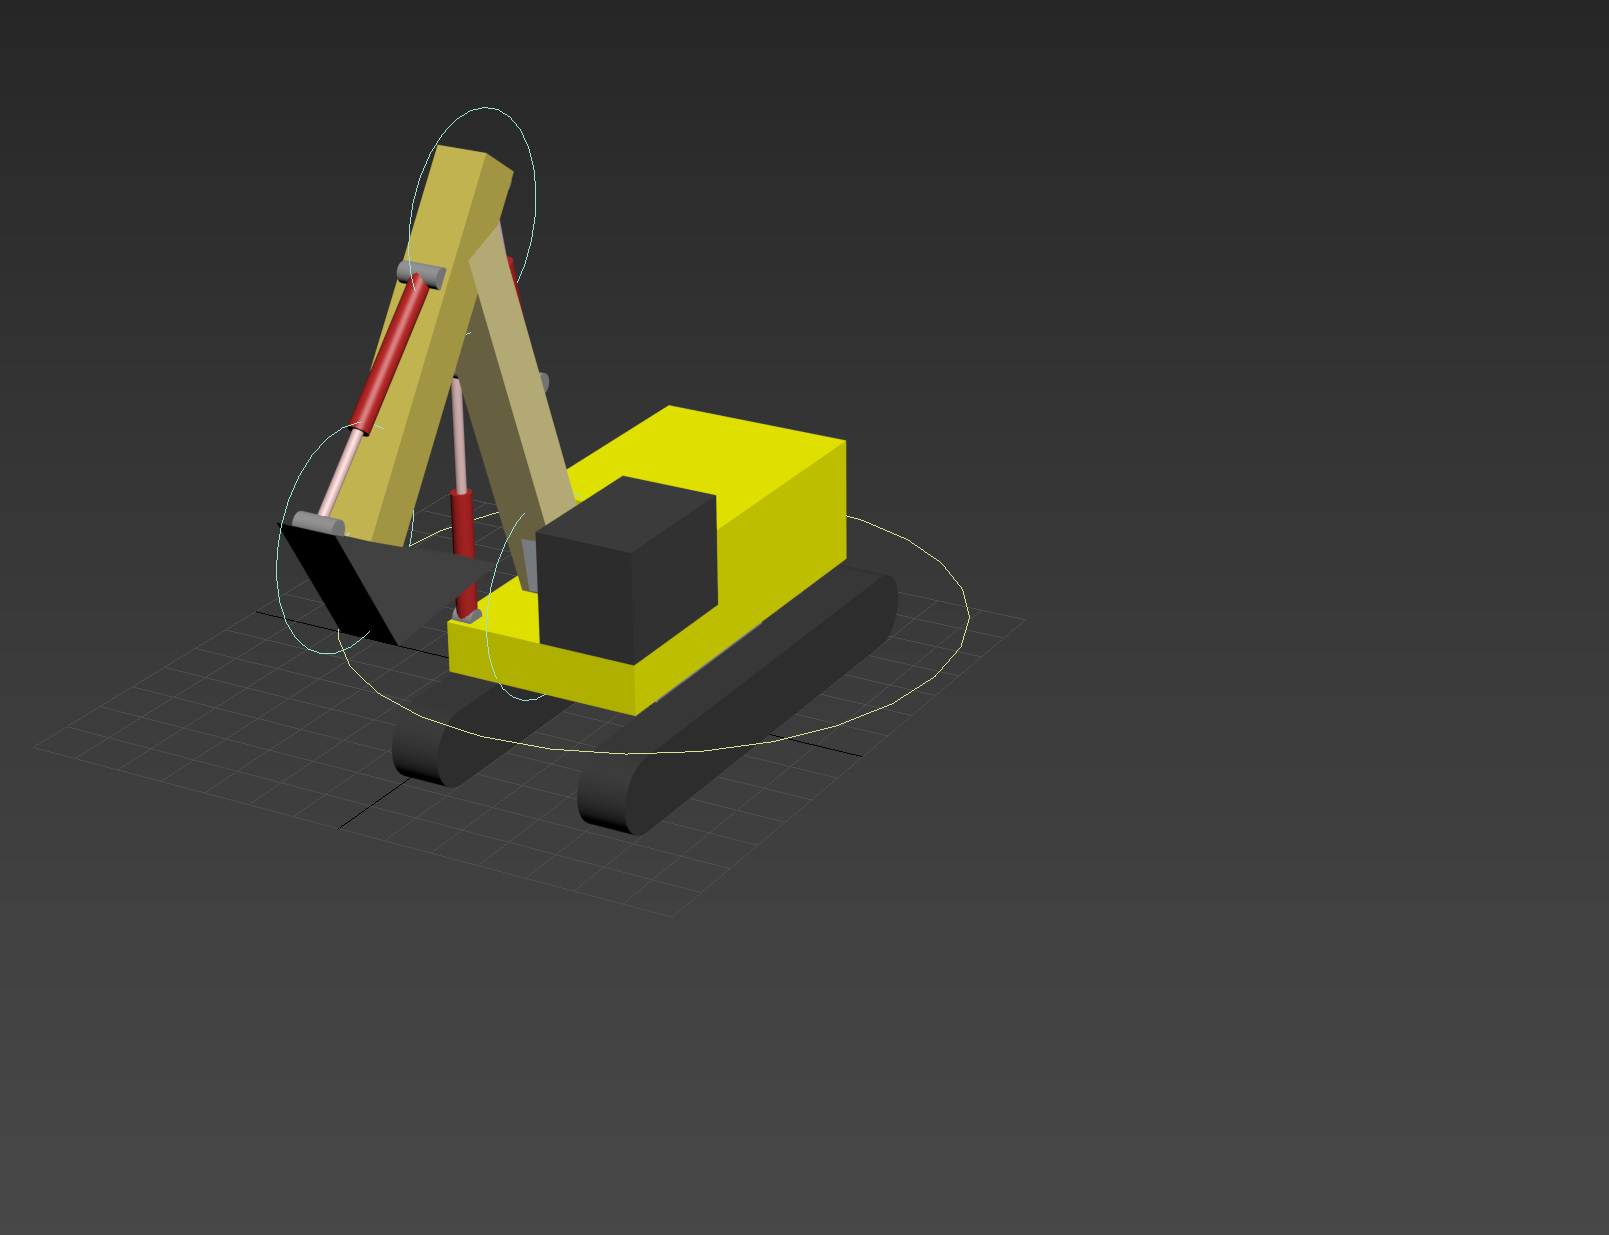
\includegraphics[width=\textwidth]{imagenes/animacion/0.png}
        \caption{Excavadora en el instante 0.}
    \end{subfigure}
    \hfill
    %\par\bigskip %si se desea dejar un margen entre la imagen de arriba y de abajo. SOLO SE PUEDE USAR HFILL O ESTE
    %\hspace{10px} %si se quiere poner una medida personalizada
	\begin{subfigure}[t]{0.48\textwidth}
	    \centering
	    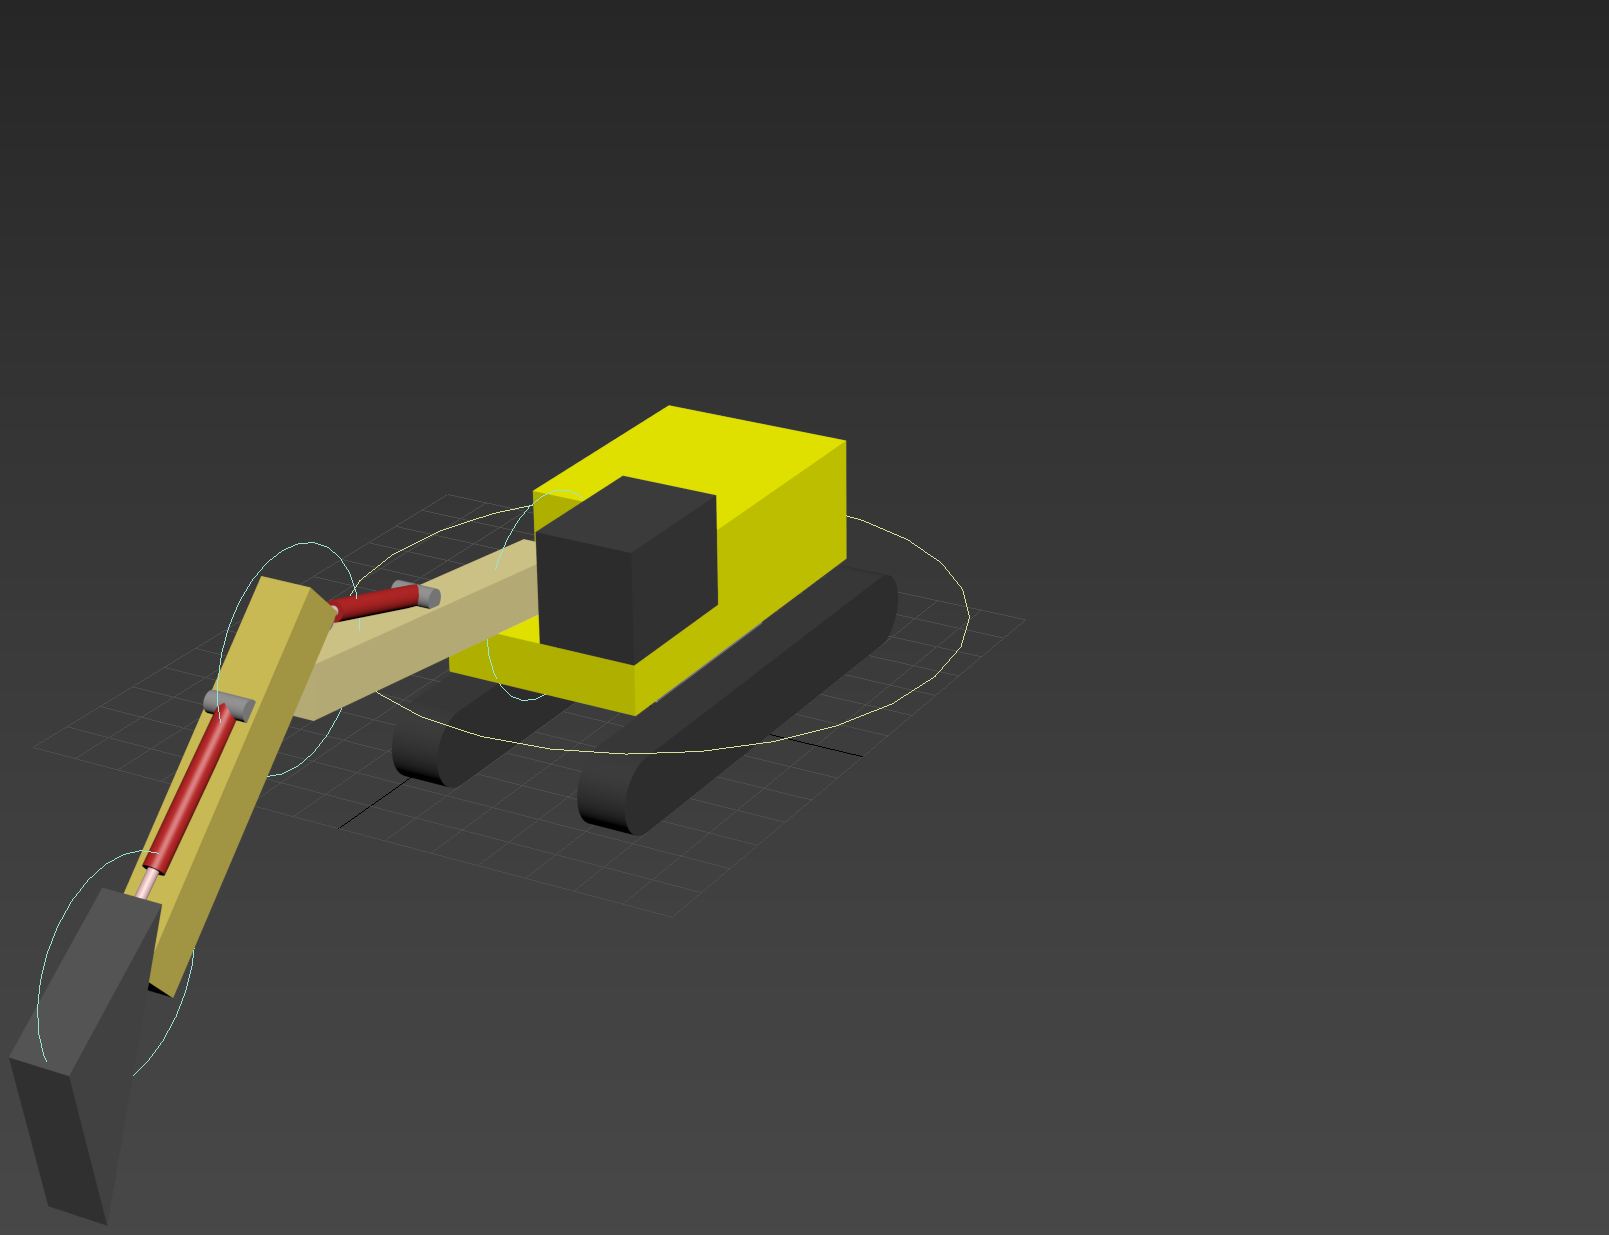
\includegraphics[width=\textwidth]{imagenes/animacion/40.png}
        \caption{Excavadora en el instante 40.}
    \end{subfigure}
    \par\bigskip
	\begin{subfigure}[t]{0.48\textwidth}
	    \centering
	    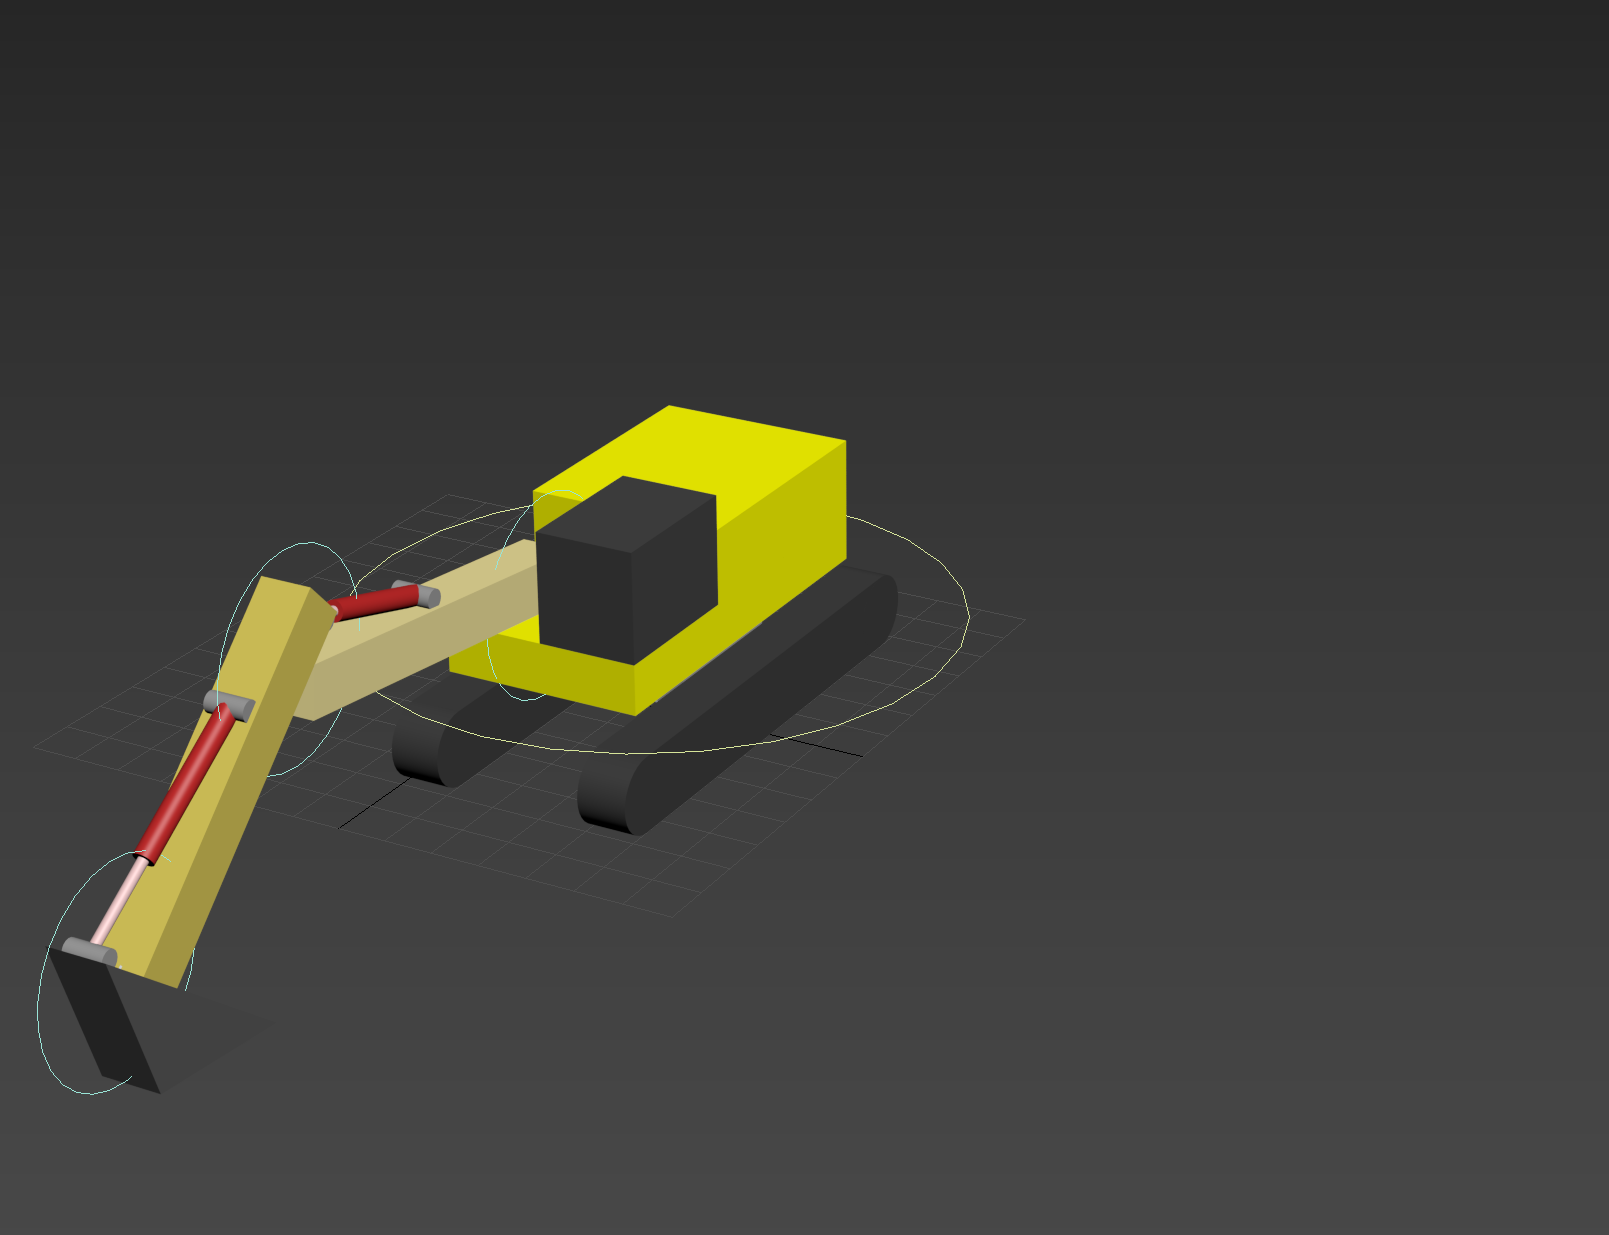
\includegraphics[width=\textwidth]{imagenes/animacion/70.png}
        \caption{Excavadora en el instante 70.}
    \end{subfigure}        
    \hfill
	\begin{subfigure}[t]{0.48\textwidth}
	    \centering
	    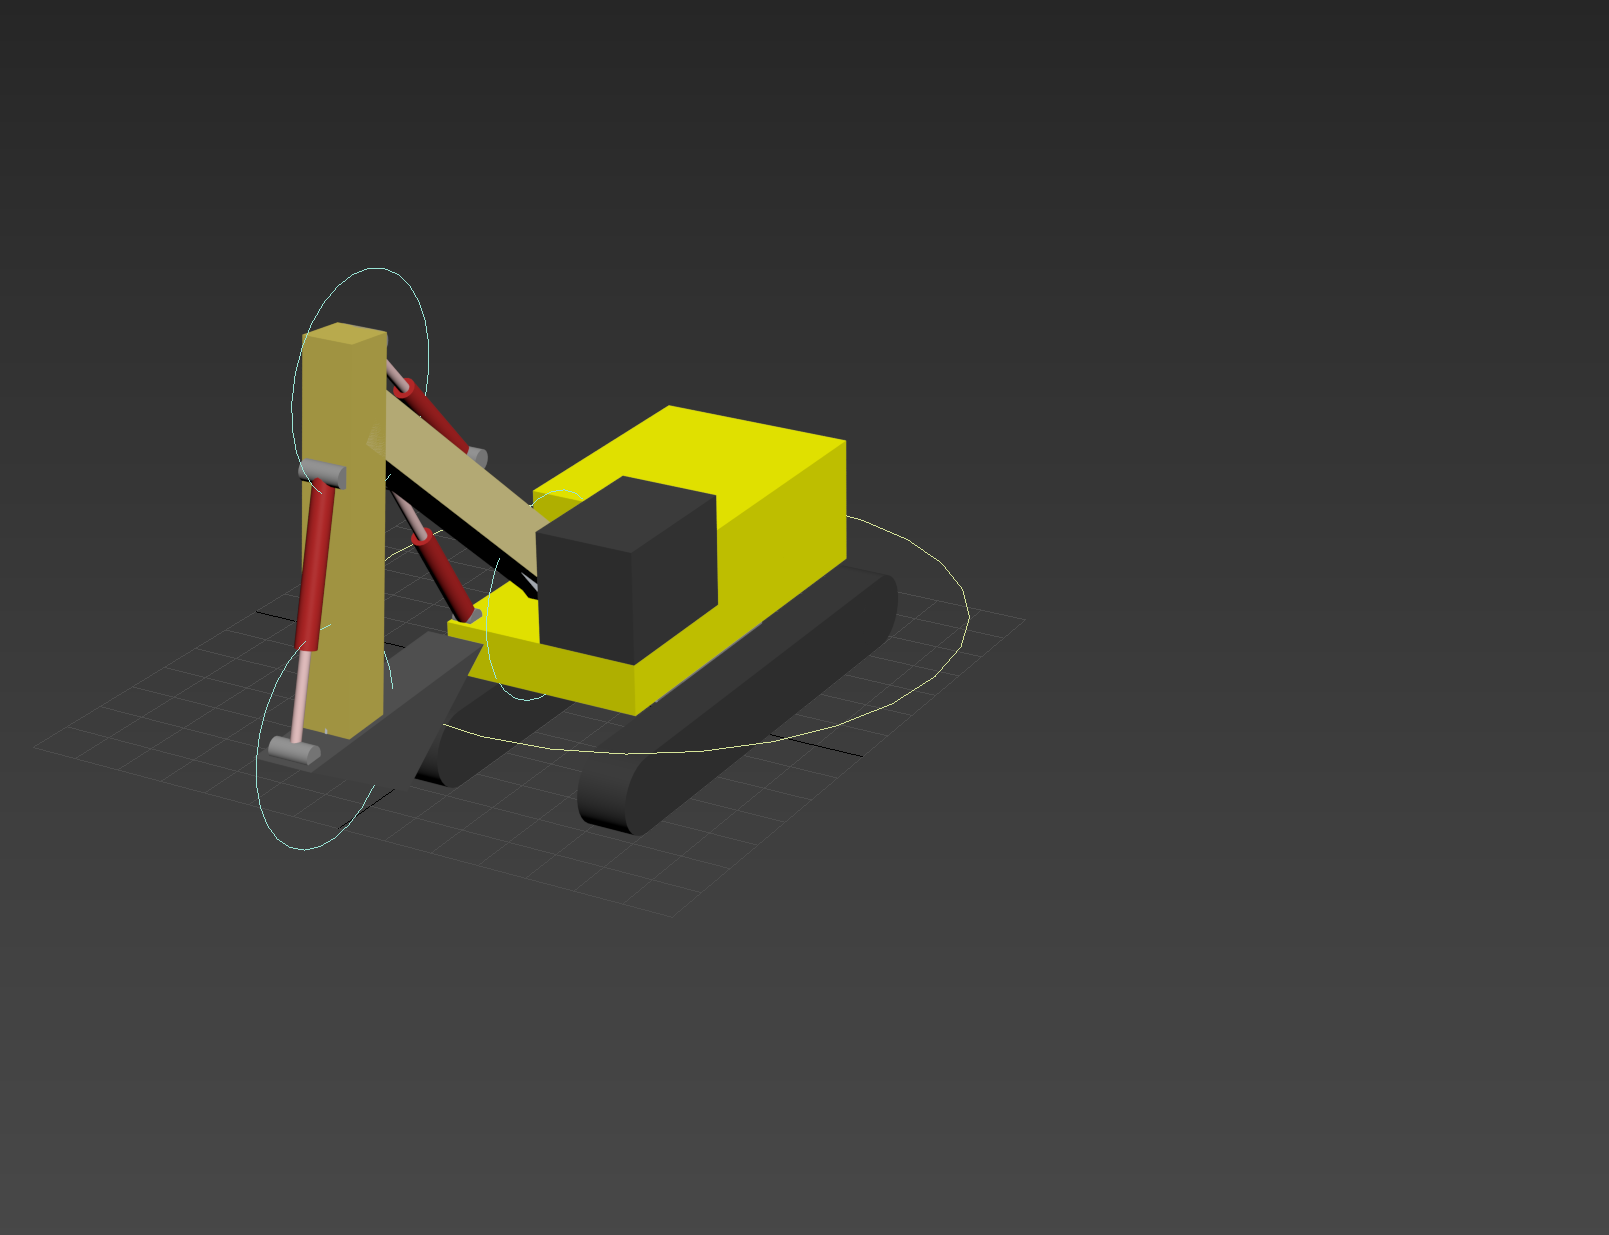
\includegraphics[width=\textwidth]{imagenes/animacion/110.png}
        \caption{Excavadora en el instante 110.}
    \end{subfigure}
    \par\bigskip 
    %\par\bigskip %si se desea dejar un margen entre la imagen de arriba y de abajo. SOLO SE PUEDE USAR HFILL O ESTE
    %\hspace{10px} %si se quiere poner una medida personalizada
	\begin{subfigure}[t]{0.48\textwidth}
	    \centering
	    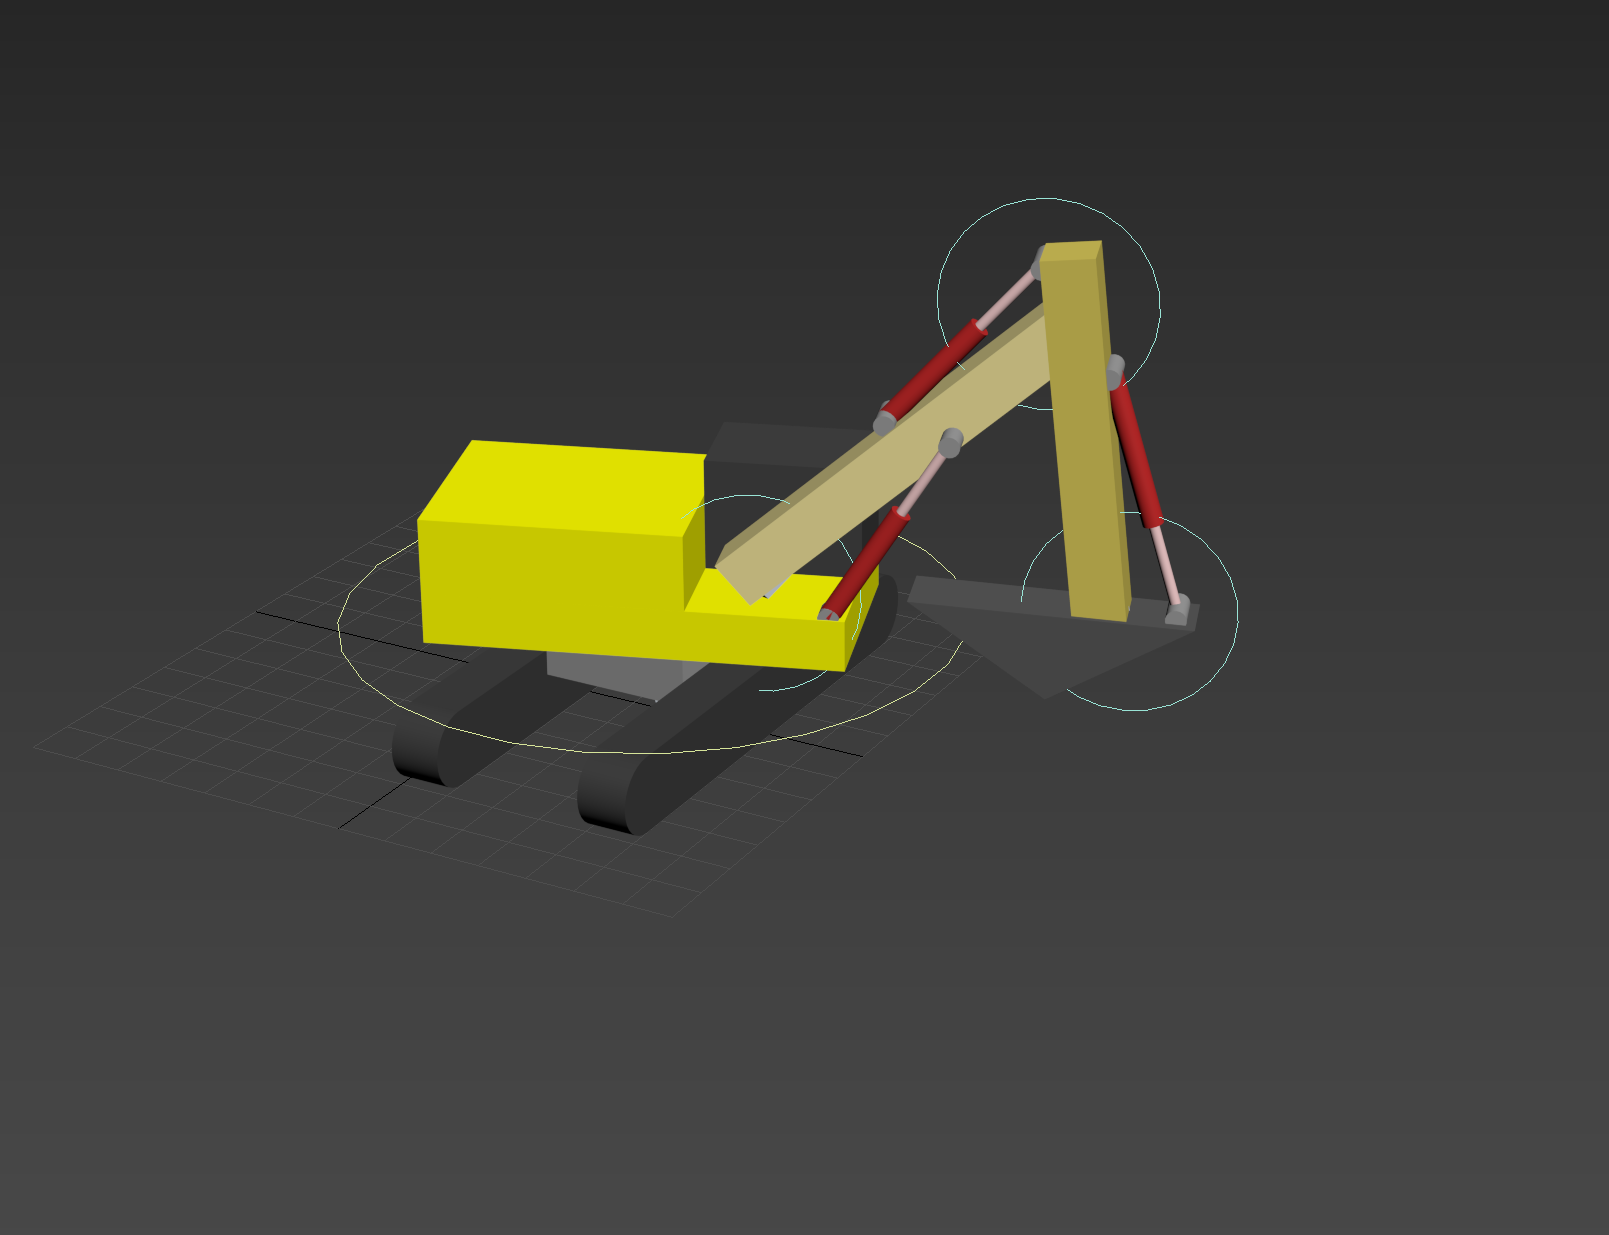
\includegraphics[width=\textwidth]{imagenes/animacion/150.png}
        \caption{Excavadora en el instante 150.}
    \end{subfigure}
    \hfill
	\begin{subfigure}[t]{0.48\textwidth}
	    \centering
	    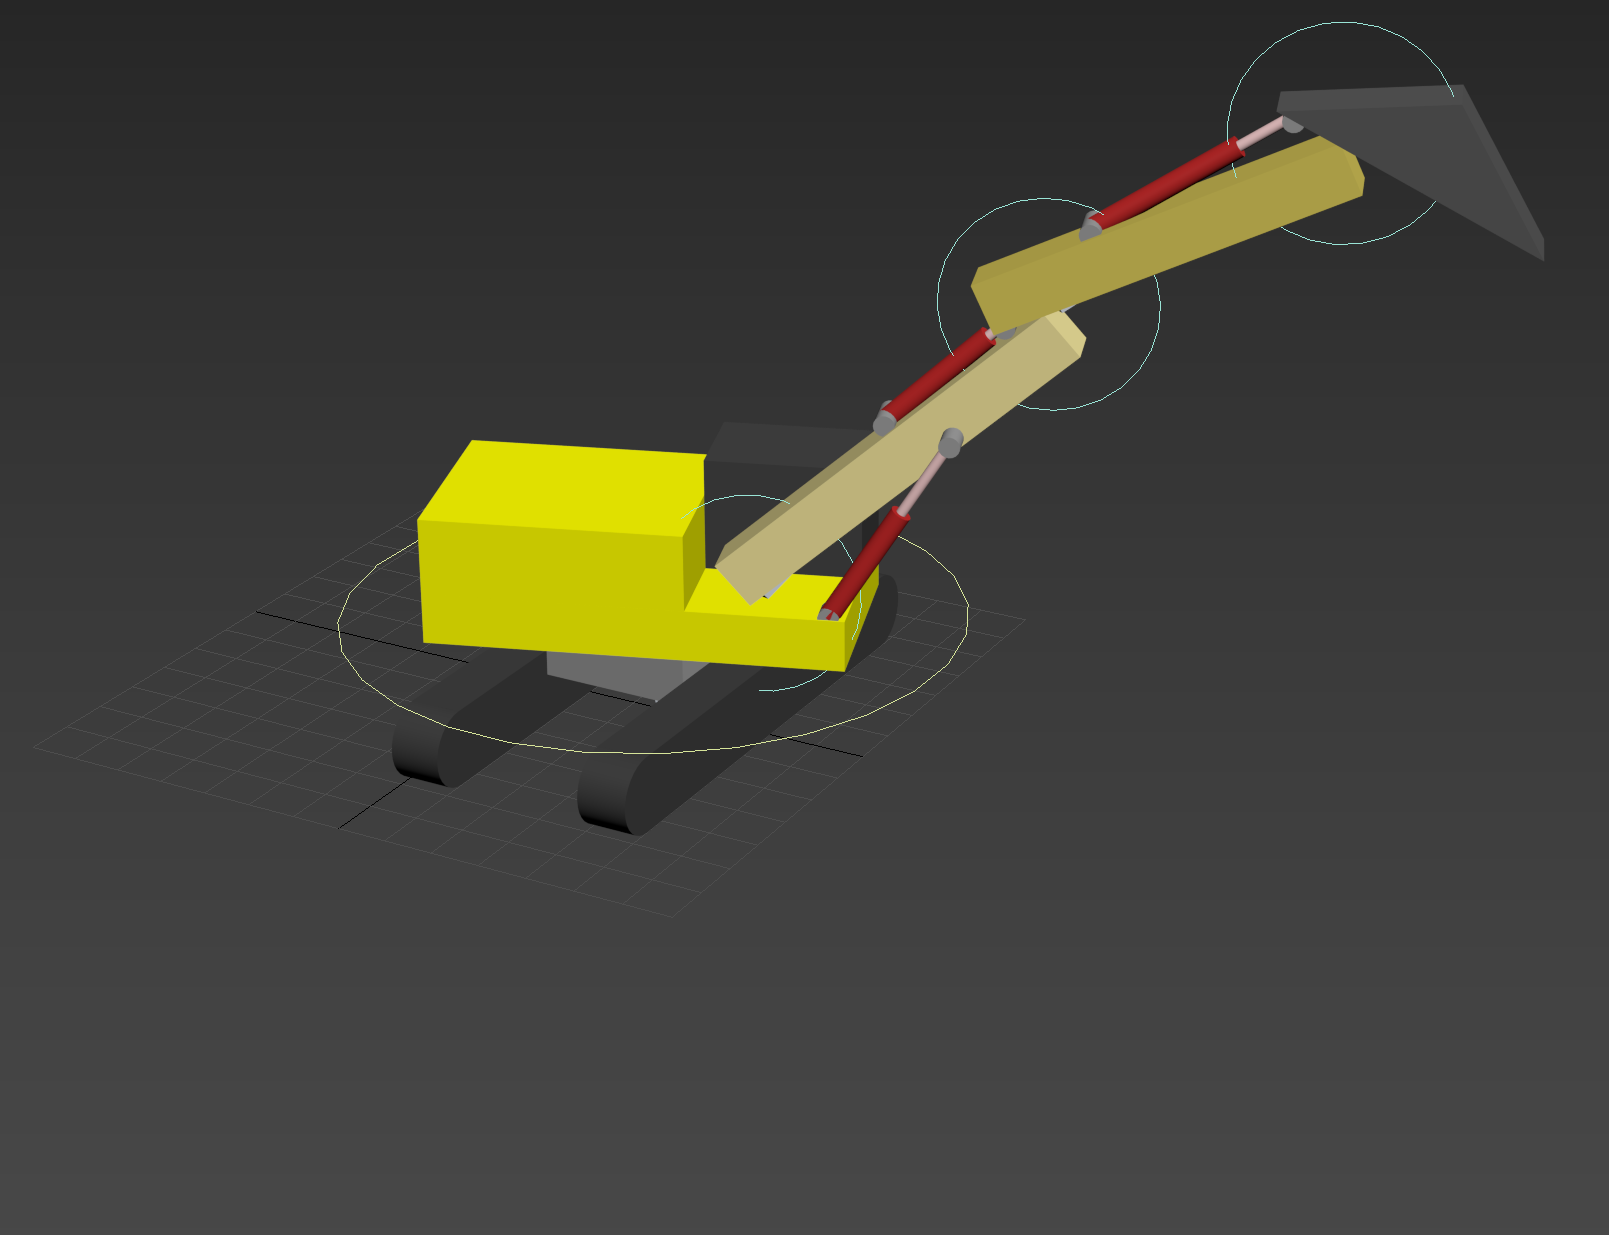
\includegraphics[width=\textwidth]{imagenes/animacion/180.png}
        \caption{Excavadora en el instante 180.}
    \end{subfigure}        
\end{figure}

\begin{figure}[H]\ContinuedFloat
\begin{subfigure}[t]{0.48\textwidth}
    \centering
    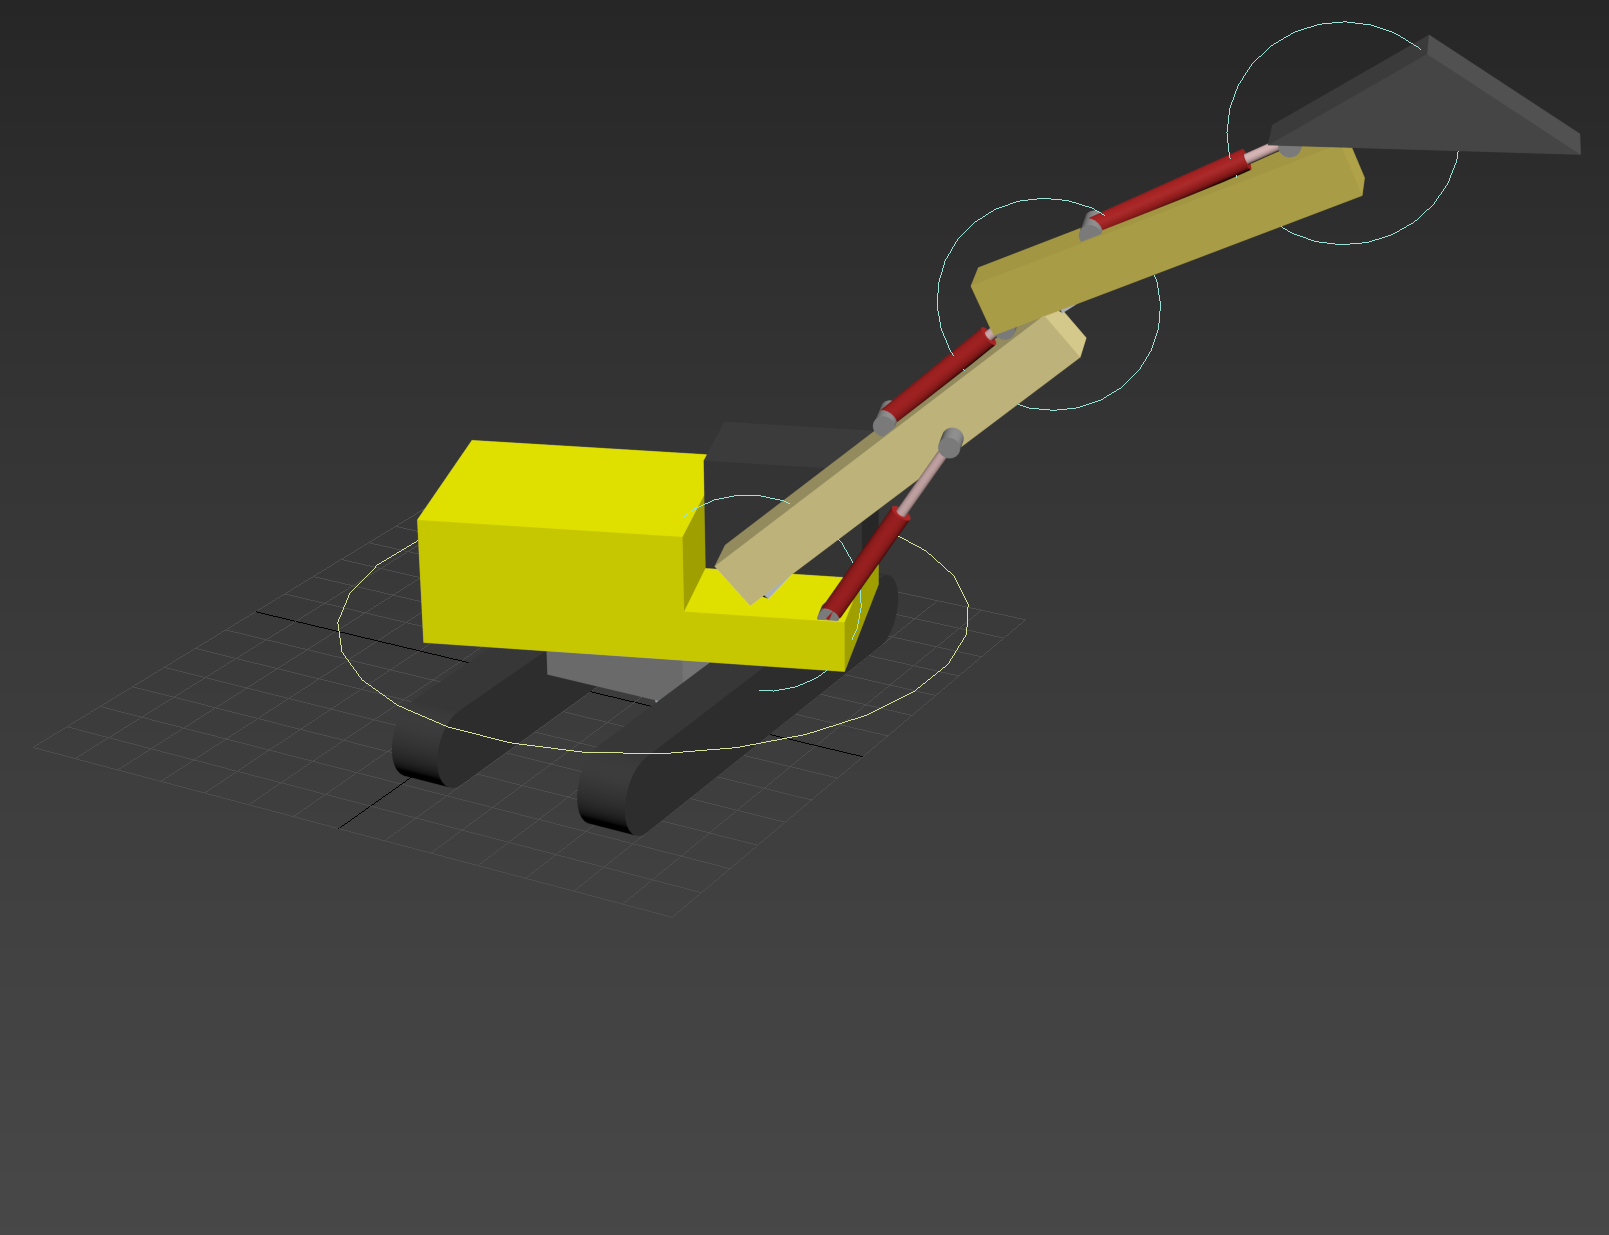
\includegraphics[width=\textwidth]{imagenes/animacion/200.png}
    \caption{Excavadora en el instante 200.}
\end{subfigure}
\hfill
%\par\bigskip %si se desea dejar un margen entre la imagen de arriba y de abajo. SOLO SE PUEDE USAR HFILL O ESTE
%\hspace{10px} %si se quiere poner una medida personalizada
\begin{subfigure}[t]{0.48\textwidth}
    \centering
    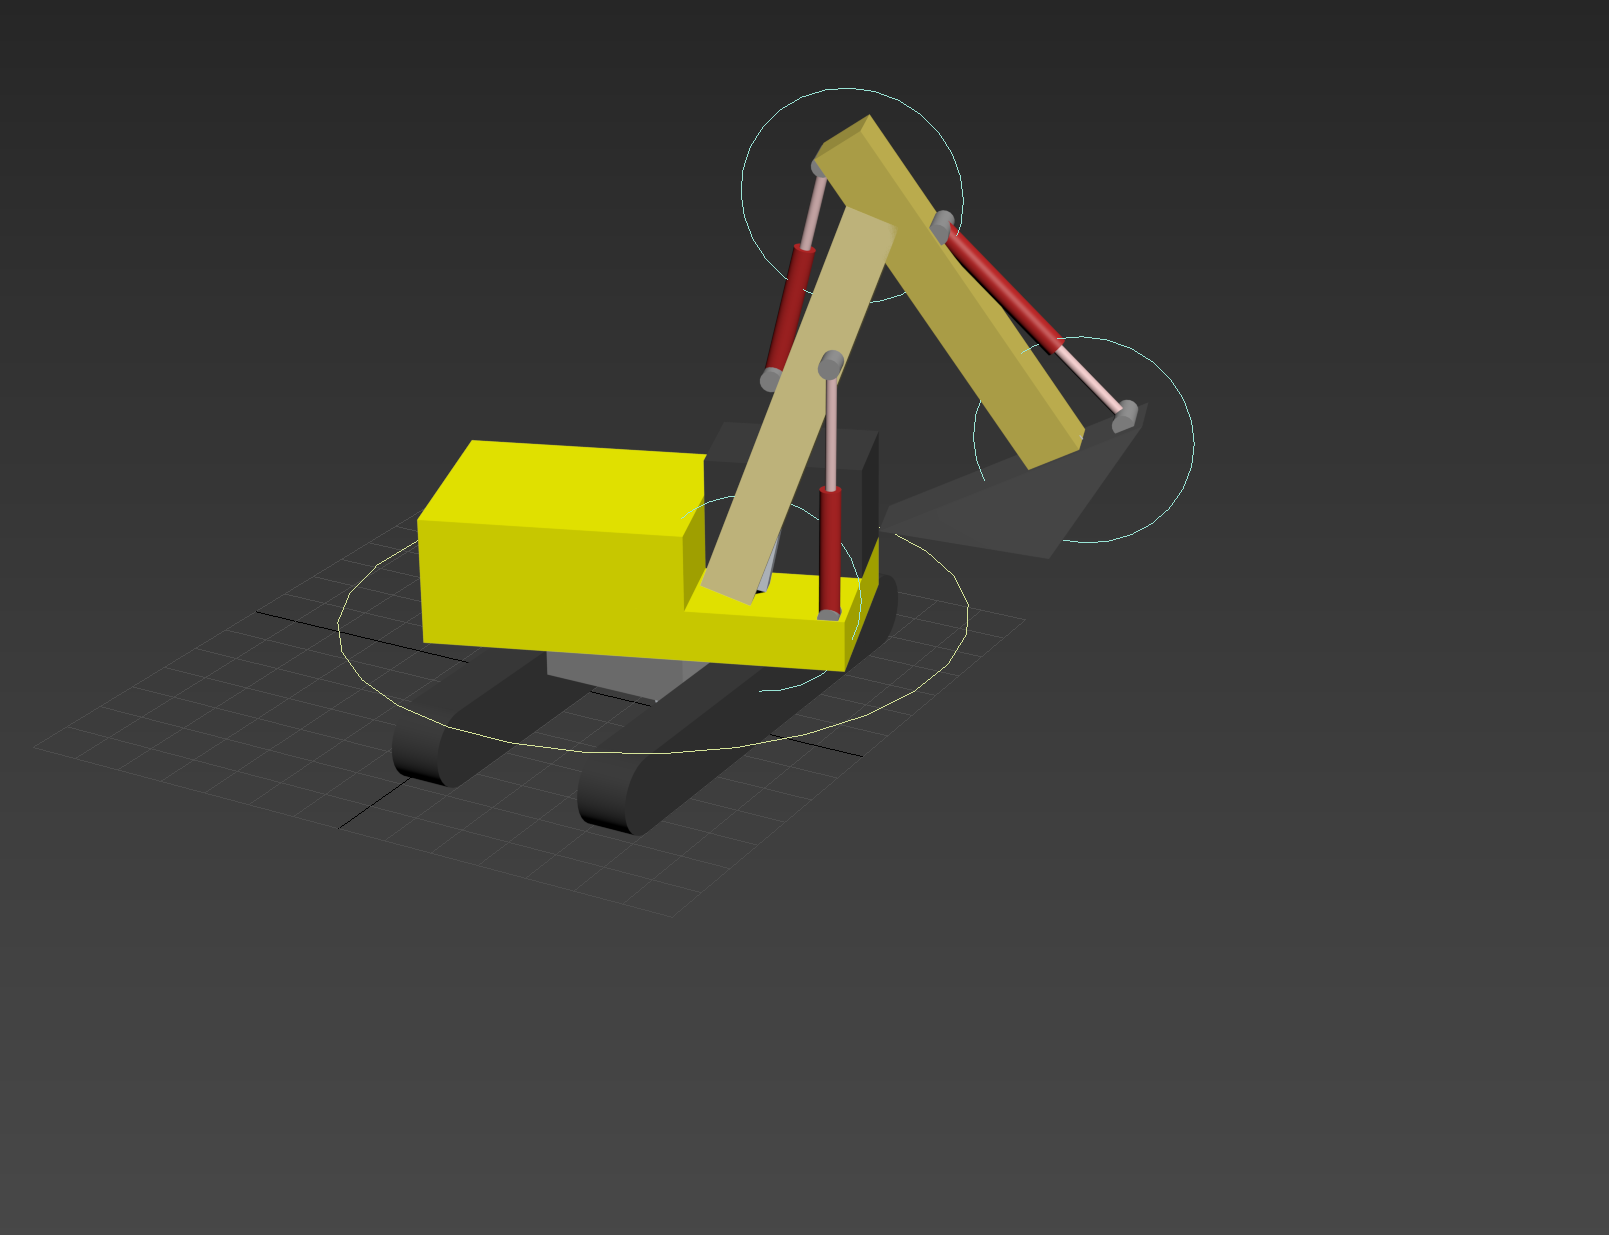
\includegraphics[width=\textwidth]{imagenes/animacion/240.png}
    \caption{Excavadora en el instante 240.}
\end{subfigure}
\par\bigskip
\begin{subfigure}[t]{\textwidth}
    \centering
    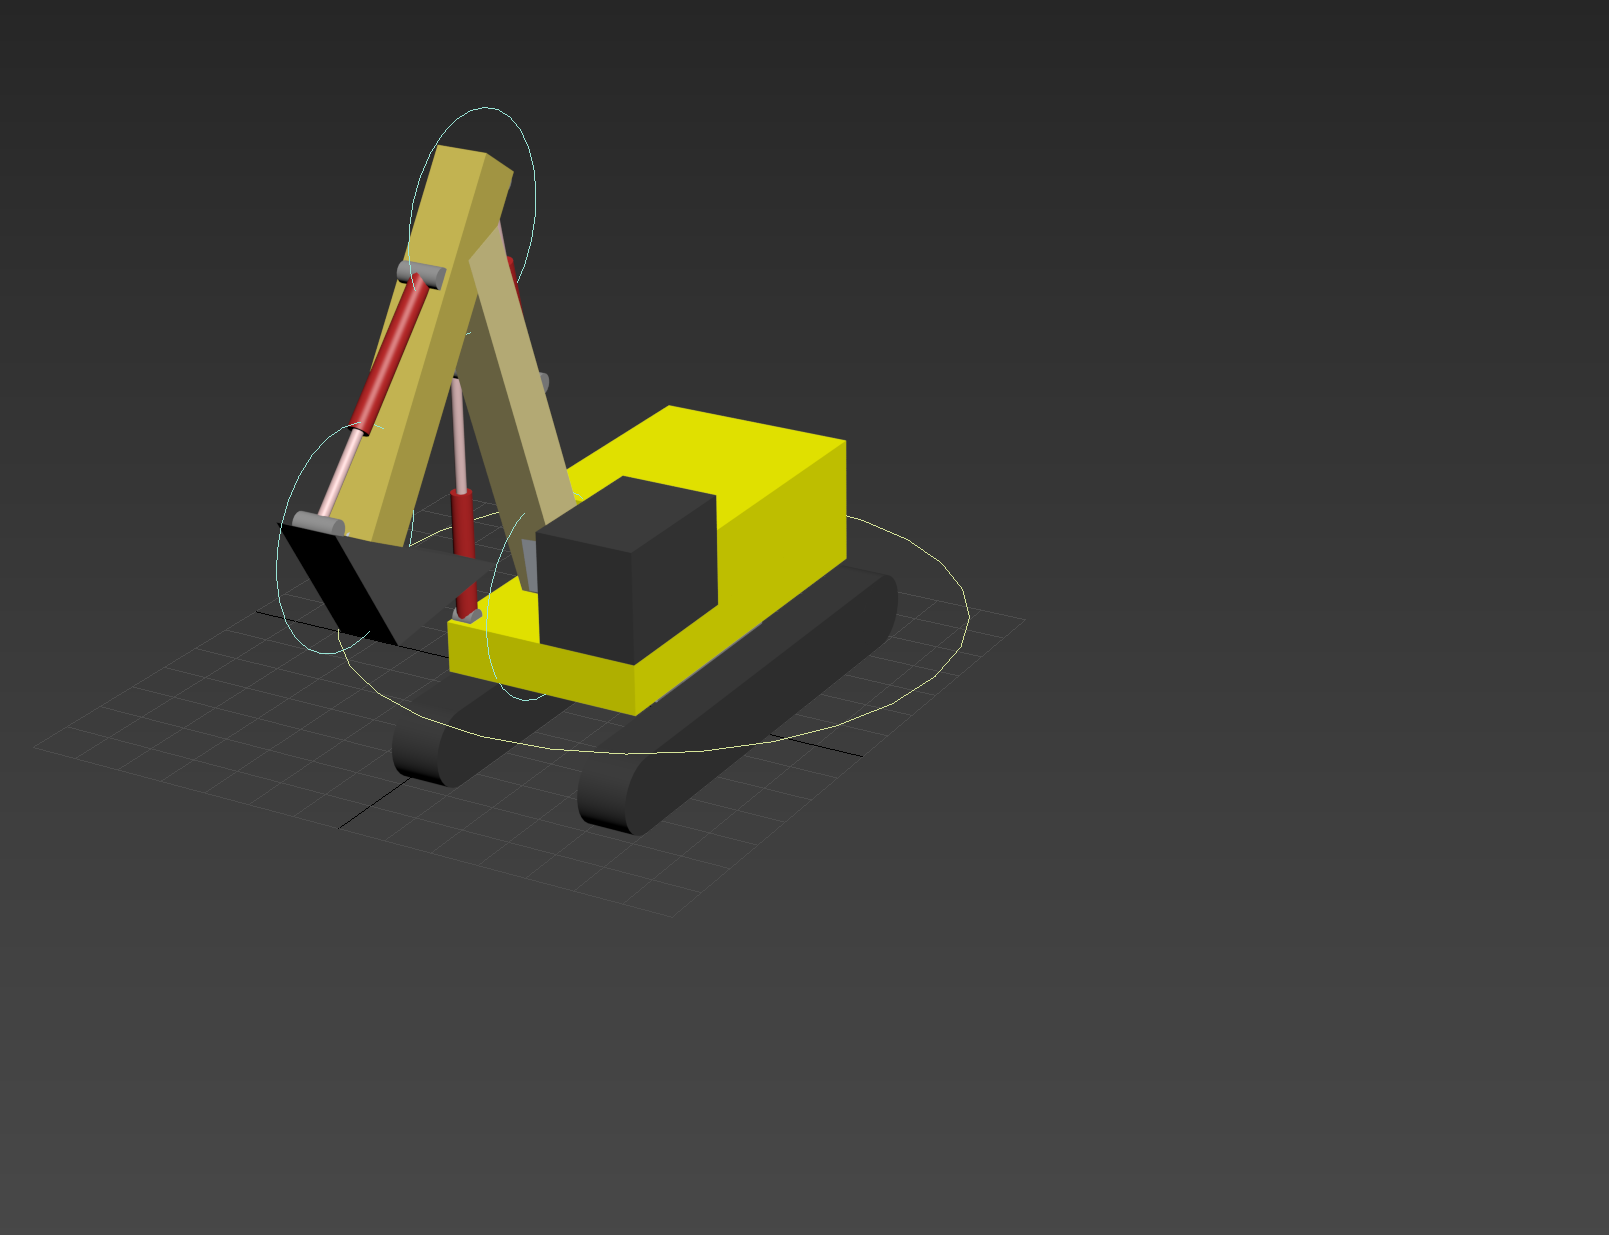
\includegraphics[width=0.48\textwidth]{imagenes/animacion/270.png}
    \caption{Excavadora en el instante 270.}
\end{subfigure}        
\caption{\textit{Keyframes} de la animación de la excavadora.}        
\end{figure}

Mientras que para las curvas de animación de los \textit{sliders}, he decidido utilizar el tipo de curva \textit{Slow-in/Slow-out}, ya que es el que me ha parecido más realista de todos, ya que el brazo necesita unos instantes para llegar a la velocidad y otros instantes para parar.